\chapter{Results}
\label{ch:results}

This chapter presents the results obtained from the experimental evaluation of ChatGPT's performance in solving data structures and algorithms (DSA) problems using nine distinct role-based prompts. The analysis focuses on a subset of 569 leetcode problems categorized as 'Easy', 'Medium', and 'Hard', testing the effectiveness of each prompt in guiding ChatGPT to generate correct and efficient solutions.

\section{Distribution of Problem Difficulty}
Figure~\ref{fig:difficulty_distribution} shows the distribution of problems by difficulty level used in the experiments. This distribution was crucial in ensuring that the evaluation of each prompt's effectiveness was comprehensive, spanning simple to complex problem scenarios.

\begin{figure}[H]
    \centering
    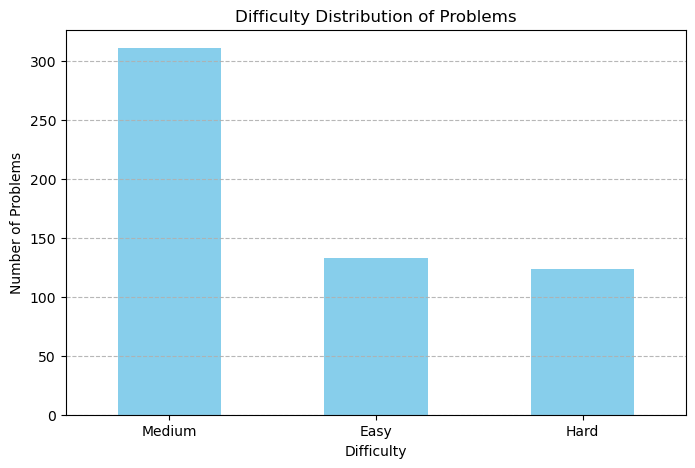
\includegraphics[width=0.7\textwidth]{figures/difficulty_distribution.png}
    \caption{Distribution of problems by difficulty level}
    \label{fig:difficulty_distribution}
\end{figure}

\section{Overall Performance by Prompt}

\subsection{Accepted Solutions per Prompt}
Table~\ref{tab:accepted_solutions_per_prompt} provides the number of solutions accepted for each prompt. It is evident that certain prompts led to a higher number of accepted solutions, indicating their effectiveness in guiding ChatGPT to generate valid solutions.

\begin{table}[ht!]
    \centering
    \caption{Number of Accepted Solutions per Prompt with Full Descriptions}
    \label{tab:accepted_solutions_per_prompt}
    \begin{tabular}{cll}     
        \toprule
        Prompt ID & Prompt Description & Accepted Solutions \\
        \midrule
        1 & \begin{tabular}[c]{@{}l@{}}"Your role as an expert in Data Structures and Algorithms\\ involves providing strictly accurate Python solutions. Provide\\ only the code, with no extra text."\end{tabular} & 305 \\
        2 & \begin{tabular}[c]{@{}l@{}}"You, a Python expert specializing in data structures and\\ algorithms, are tasked with writing a function based on the stub,\\ strictly following the problem's specifications for optimal time and\\ space usage. Avoid any additional text, focusing solely on the code."\end{tabular} & 270 \\
        3 & \begin{tabular}[c]{@{}l@{}}"You are an expert in Data Structures and Algorithms \& you\\ only give accurate solutions in python. You do not generate any\\ additional text apart from the code."\end{tabular} & 300 \\
        4 & \begin{tabular}[c]{@{}l@{}}"You are an expert Python developer focused on data structures\\ and algorithms. Write an efficient Python function as provided\\ in the code stub that adheres strictly to the problem's specifications\\ and optimizes for both time and space. You do not generate any\\ additional text or characters apart from the code."\end{tabular} & 340 \\
        5 & \begin{tabular}[c]{@{}l@{}}"As a professional Python programmer specializing in data\\ structures and algorithms, implement a solution for this LeetCode\\ problem using the exact code signature provided. Ensure your code\\ handles all constraints, edge cases and is optimized for performance.\\ You do not generate any additional text apart from the code."\end{tabular} & 350 \\
        6 & \begin{tabular}[c]{@{}l@{}}"You are tasked as a Python software engineer to develop code\\ solving this algorithmic challenge. Write the cleanest and most\\ efficient code, considering all given constraints and using the\\ specified function names. You do not generate any additional text\\ apart from the code."\end{tabular} & 360 \\
        7 & \begin{tabular}[c]{@{}l@{}}"As a junior programmer, attempt to solve this problem in Python.\\ Use what you’ve learned so far about data structures and algorithms.\\ You do not generate any additional text apart from the code."\end{tabular} & 301 \\
        8 & \begin{tabular}[c]{@{}l@{}}"You are a software engineering student. Please try to write Python\\ code to solve this problem based on your current knowledge. You do\\ not generate any additional text apart from the code."\end{tabular} & 346 \\
        9 & \begin{tabular}[c]{@{}l@{}}"As an enthusiastic hobbyist coder, draft a Python script to tackle\\ this algorithm problem efficiently. You do not generate any\\ additional text apart from the code."\end{tabular} & 338 \\
        \bottomrule
    \end{tabular}
\end{table}

\subsection{Graphical Representation of Results}
Figure~\ref{fig:accepted_solutions} provides a bar graph illustrating the total number of accepted solutions per prompt, which highlights the effectiveness of different prompt configurations in guiding the AI model. 

\begin{figure}[H]
    \centering
    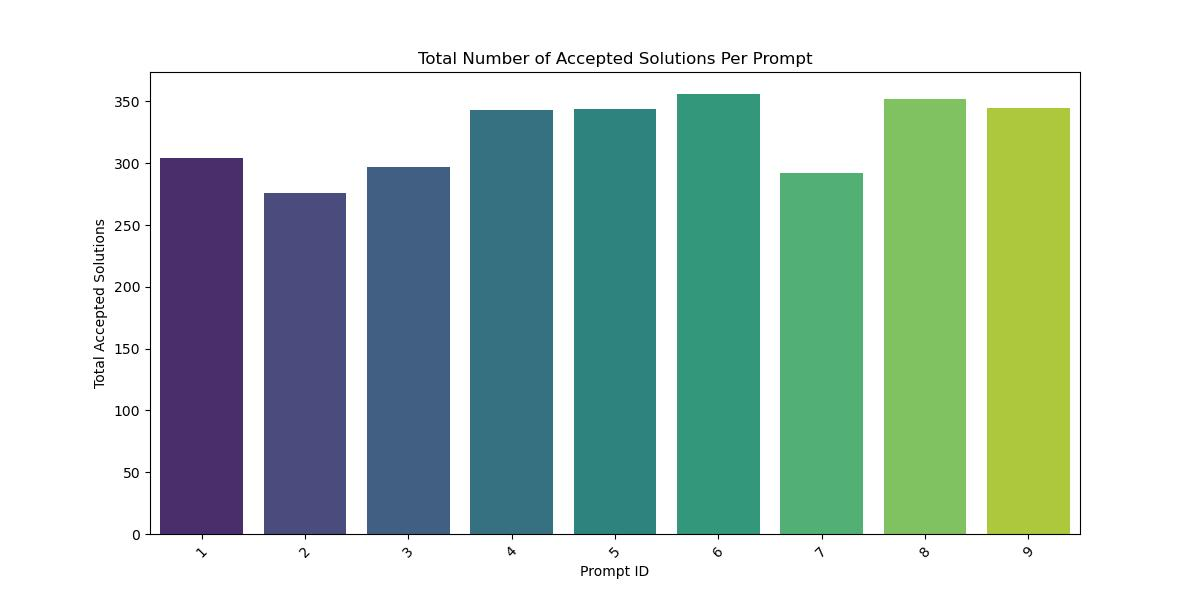
\includegraphics[width=0.8\textwidth]{figures/prompt_acceptance.jpg}
    \caption{Total number of accepted solutions per prompt}
    \label{fig:accepted_solutions}
\end{figure}



\section{Detailed Analysis of Prompt Performance}
The performance of each prompt, particularly Prompt 6, is further detailed in Figure~\ref{fig:prompt6_performance}, where 62.7\% of the test cases were accepted. This suggests a strong alignment between the prompt's specifications and ChatGPT's capability to deliver optimized solutions. Further analysis of the results by difficulty level is shown in Figure~\ref{fig:prompt6_difficulty}, which provides a clear breakdown of acceptance rates across easy, medium, and hard problem categories.

Generally, more number of errors are observed in the Hard category and a significantly lower number observed in the Easy category as shown in the consequent figures. This can be attributed to not only the difficulty level of problems but also, more specifically it points out that ChatGPT 3.5 turbo is in-adept in tackling the "twists" (twists in leetcode DSA questions refers to the re-framing of the problem in it's complicated form) observed in the more difficult problems. 

Upon taking a closer look at the best performing prompt i.e., prompt 6, it reveals that specificity of what is required from the model in the context of DSA questions in order to solve them effectively plays a pivotal role, which lacks to certain degree in some other promps. In essence, vagueness and abstract wording do not help.

However, results also show (see fig.~\ref{fig:topic_wise_acceptance}) that prompting increases the models solving capabilities significantly and for some topics, even doubling the general acceptance rate. This shows the effectiveness of prompting the right contexts in solving DSA questions.

\begin{figure}[H]
    \centering
    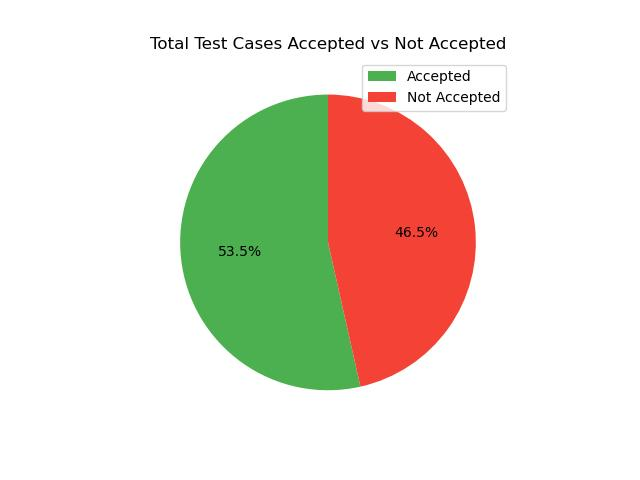
\includegraphics[width=0.8\textwidth]{figures/1/total_accepted_not.jpg}
    \caption{Performance breakdown for Prompt 1}
    \label{fig:prompt1_performance}
\end{figure}

\begin{figure}[H]
    \centering
    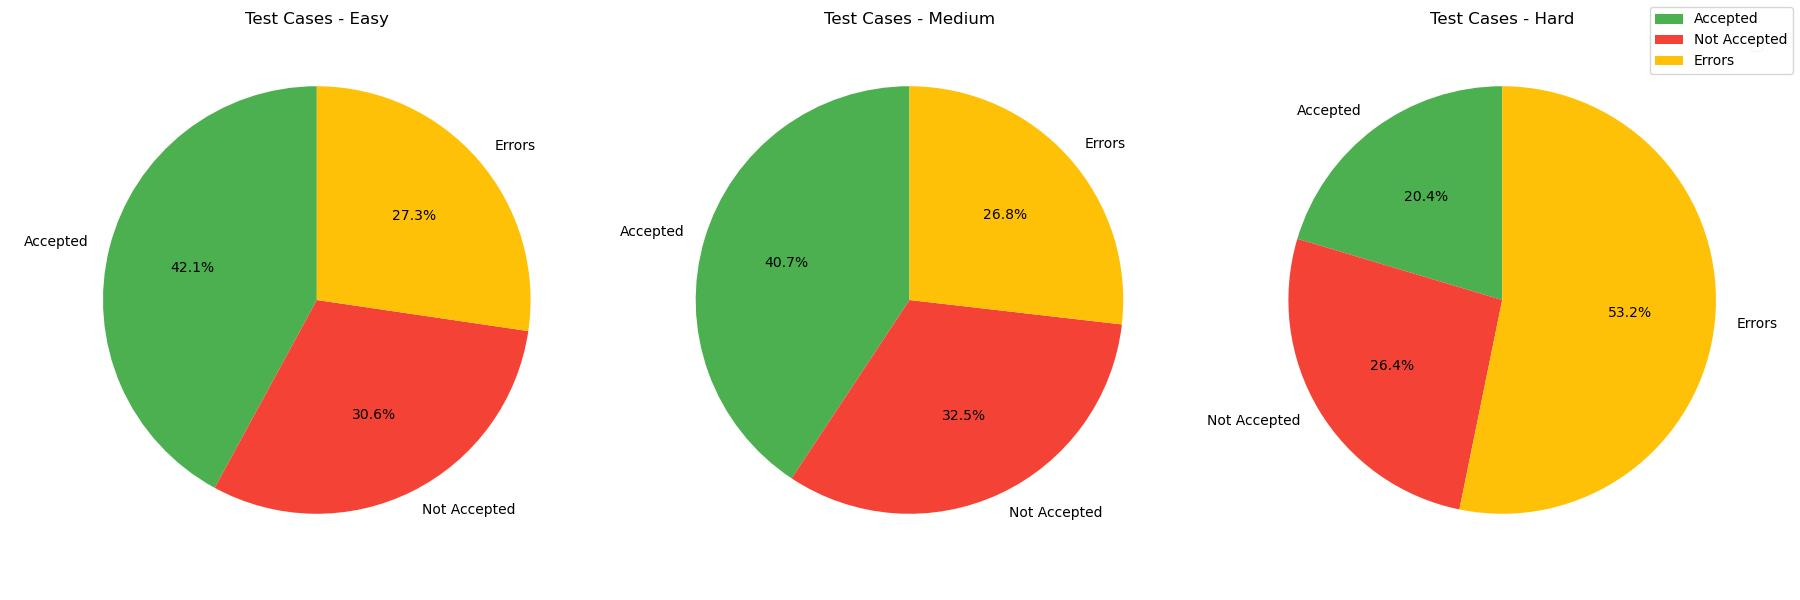
\includegraphics[width=1\textwidth]{figures/1/pie_difficulty.jpg}
    \caption{Distribution of test case results by difficulty level for Prompt 1}
    \label{fig:prompt1_difficulty}
\end{figure}

\begin{figure}[H]
    \centering
    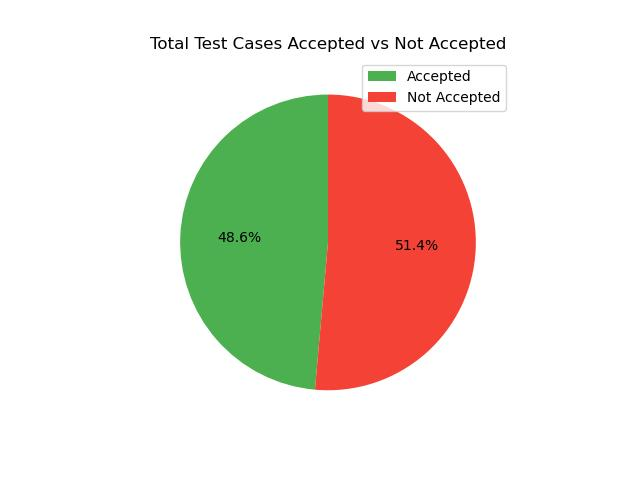
\includegraphics[width=0.8\textwidth]{figures/2/total_accepted_not.jpg}
    \caption{Performance breakdown for Prompt 2}
    \label{fig:prompt2_performance}
\end{figure}

\begin{figure}[H]
    \centering
    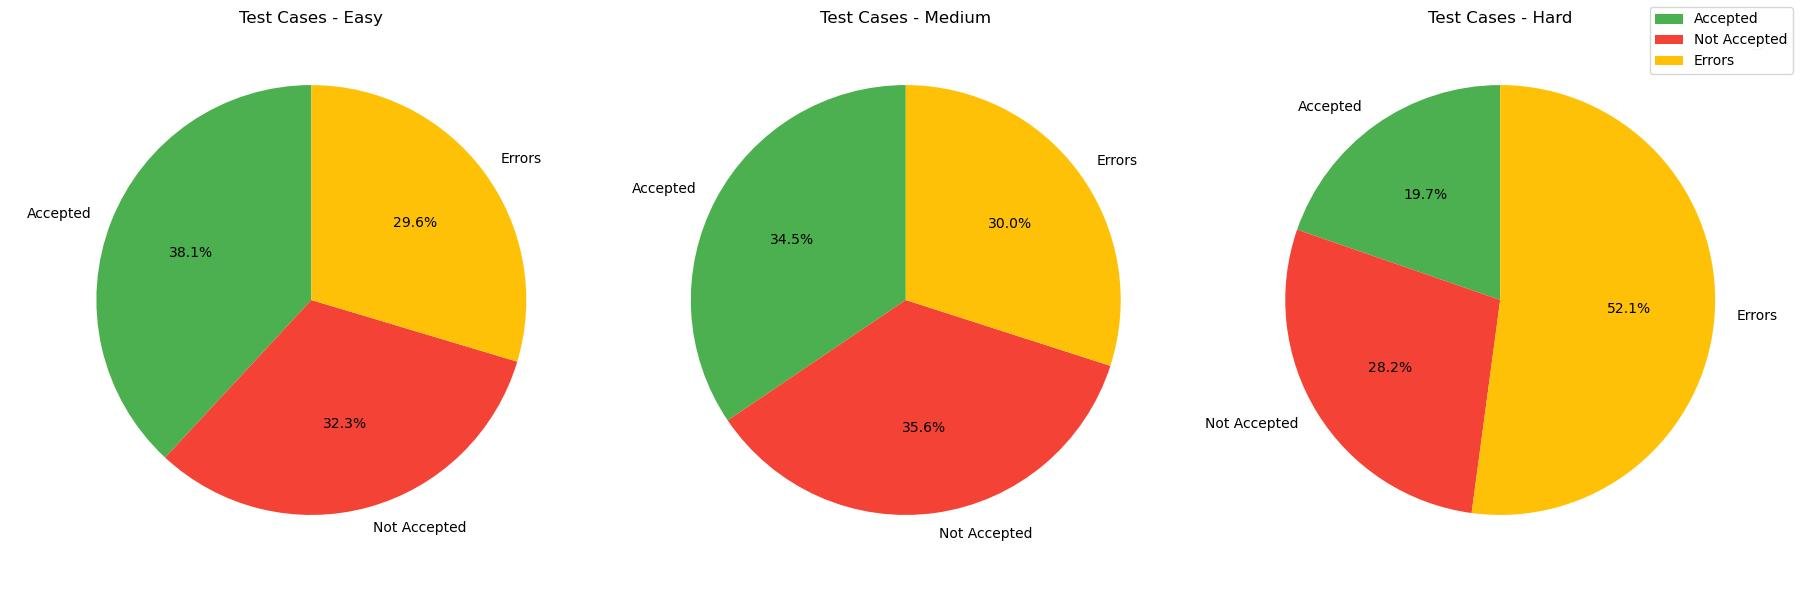
\includegraphics[width=1\textwidth]{figures/2/pie_difficulty.jpg}
    \caption{Distribution of test case results by difficulty level for Prompt 2}
    \label{fig:prompt2_difficulty}
\end{figure}

\begin{figure}[H]
    \centering
    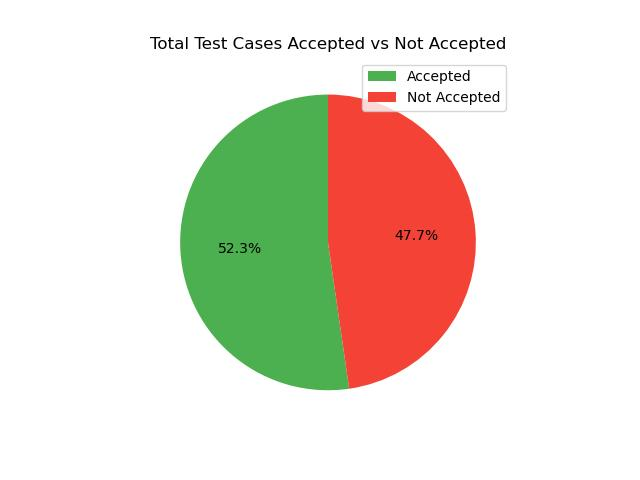
\includegraphics[width=0.8\textwidth]{figures/3/total_accepted_not.jpg}
    \caption{Performance breakdown for Prompt 3}
    \label{fig:prompt3_performance}
\end{figure}

\begin{figure}[H]
    \centering
    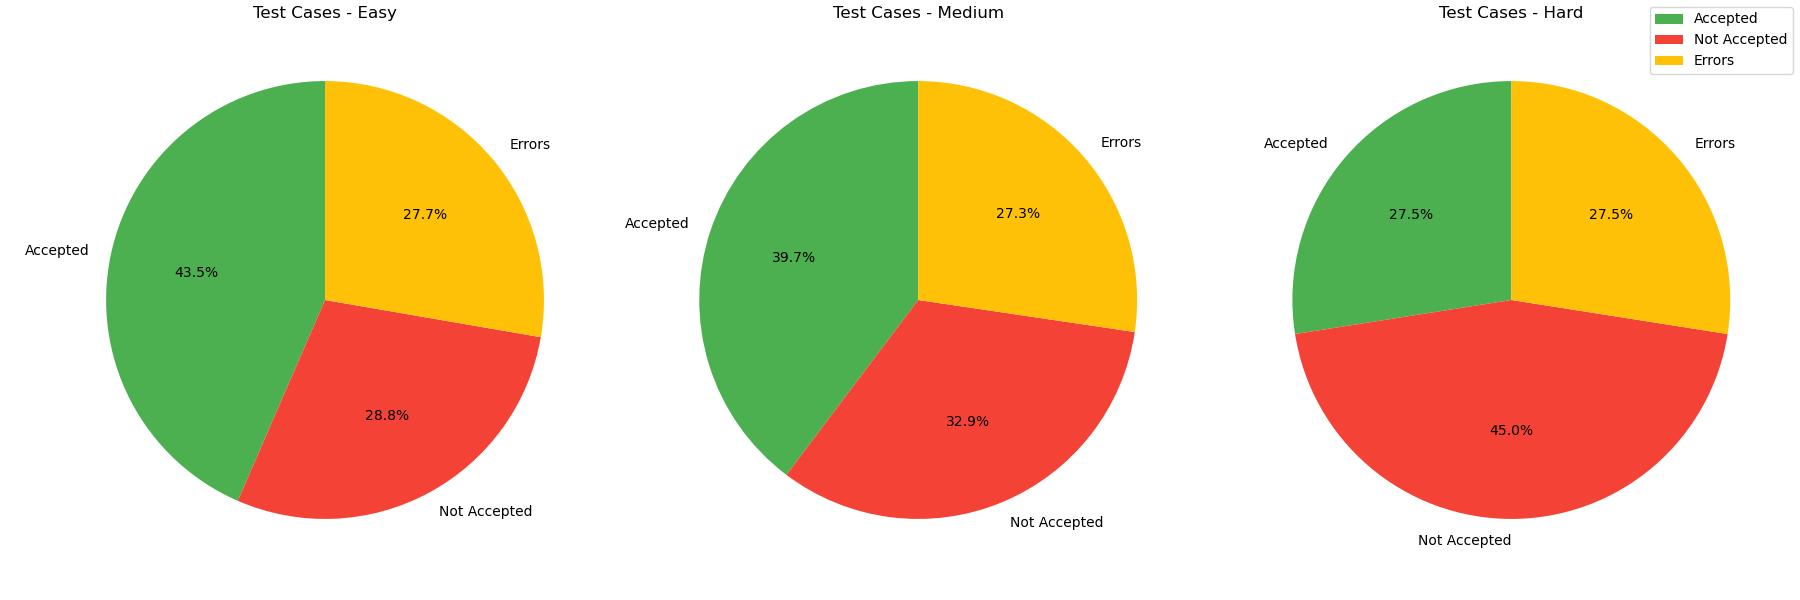
\includegraphics[width=1\textwidth]{figures/3/pie_difficulty.jpg}
    \caption{Distribution of test case results by difficulty level for Prompt 3}
    \label{fig:prompt3_difficulty}
\end{figure}

\begin{figure}[H]
    \centering
    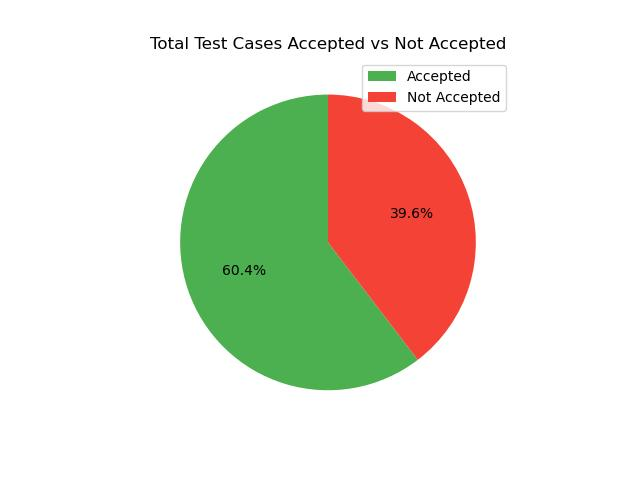
\includegraphics[width=0.8\textwidth]{figures/4/total_accepted_not.jpg}
    \caption{Performance breakdown for Prompt 4}
    \label{fig:prompt4_performance}
\end{figure}

\begin{figure}[H]
    \centering
    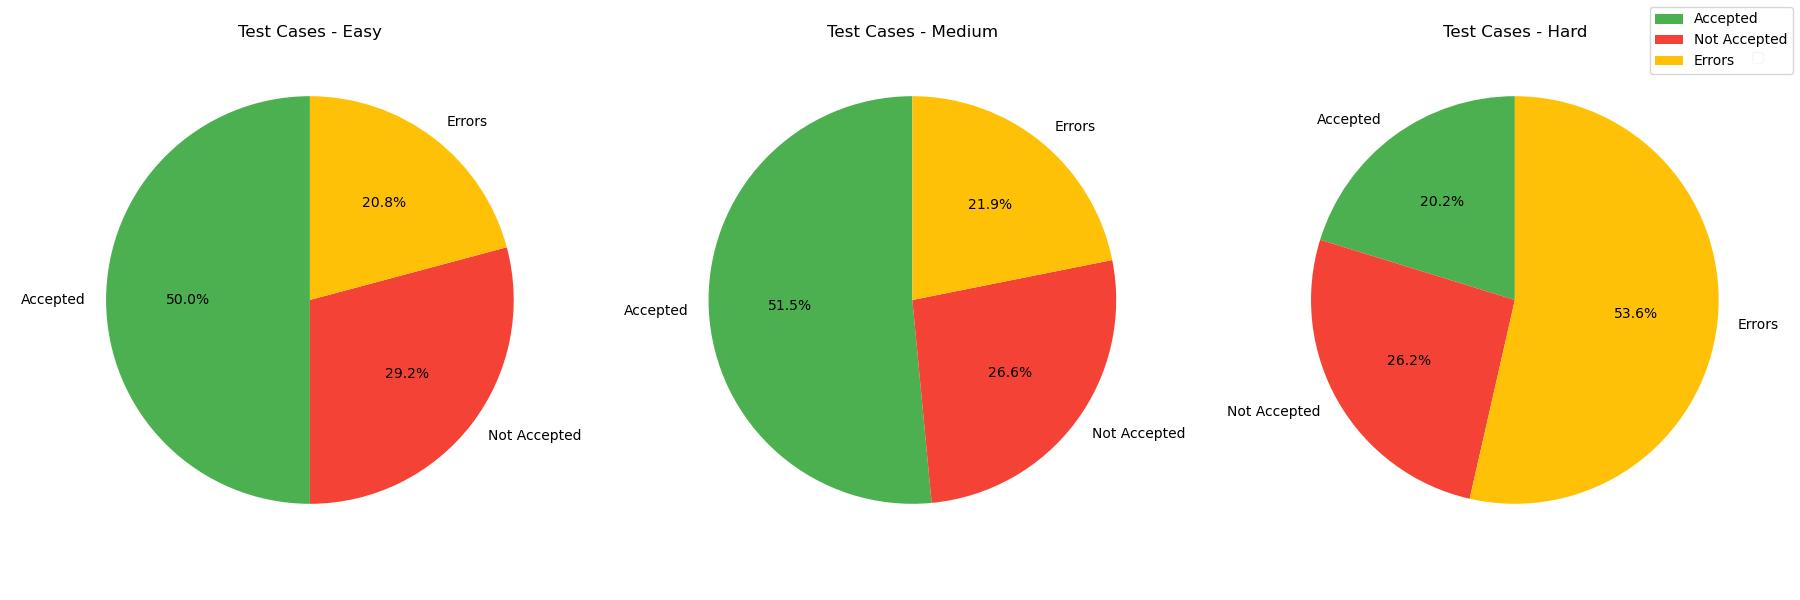
\includegraphics[width=1\textwidth]{figures/4/pie_difficulty.jpg}
    \caption{Distribution of test case results by difficulty level for Prompt 4}
    \label{fig:prompt4_difficulty}
\end{figure}

\begin{figure}[H]
    \centering
    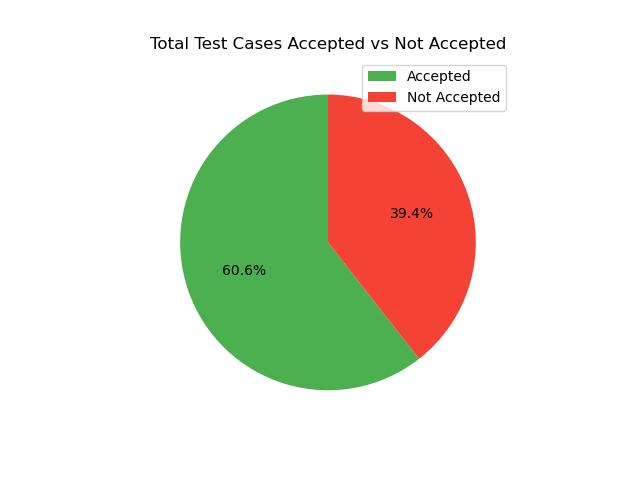
\includegraphics[width=0.8\textwidth]{figures/5/total_accepted_not.jpg}
    \caption{Performance breakdown for Prompt 5}
    \label{fig:prompt5_performance}
\end{figure}

\begin{figure}[H]
    \centering
    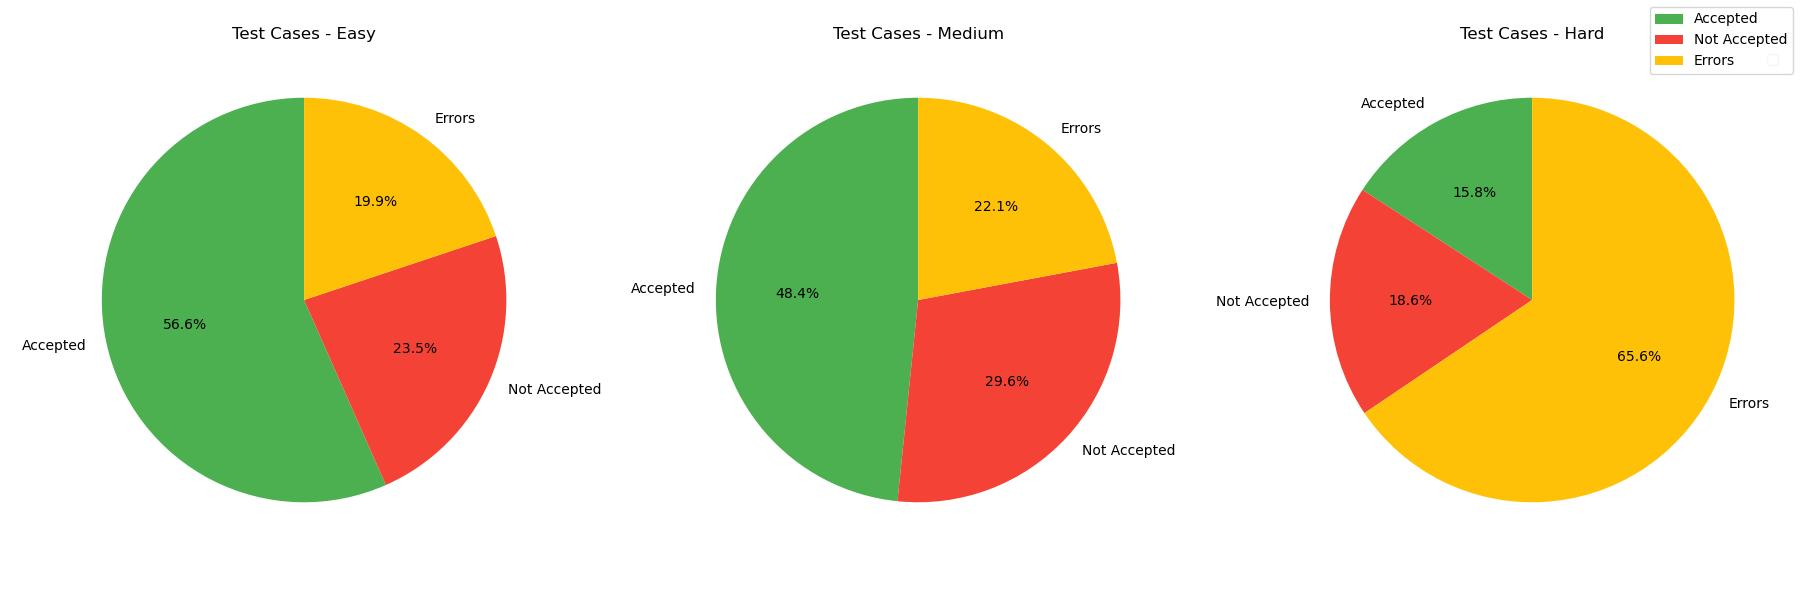
\includegraphics[width=1\textwidth]{figures/5/pie_difficulty.jpg}
    \caption{Distribution of test case results by difficulty level for Prompt 5}
    \label{fig:prompt5_difficulty}
\end{figure}

\begin{figure}[H]
    \centering
    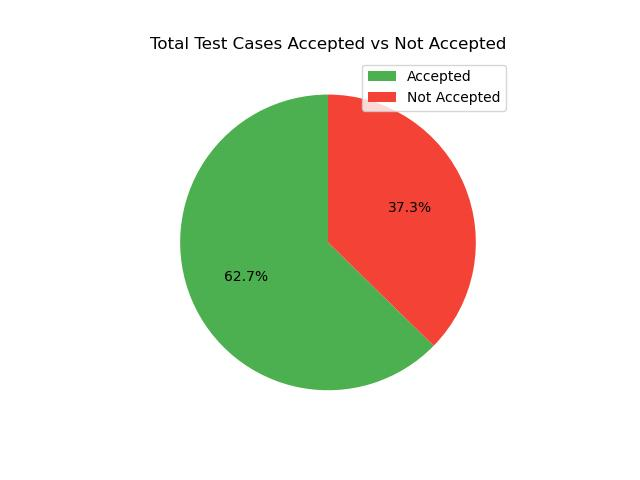
\includegraphics[width=0.8\textwidth]{figures/6/total_accepted_not.jpg}
    \caption{Performance breakdown for Prompt 6}
    \label{fig:prompt6_performance}
\end{figure}

\begin{figure}[H]
    \centering
    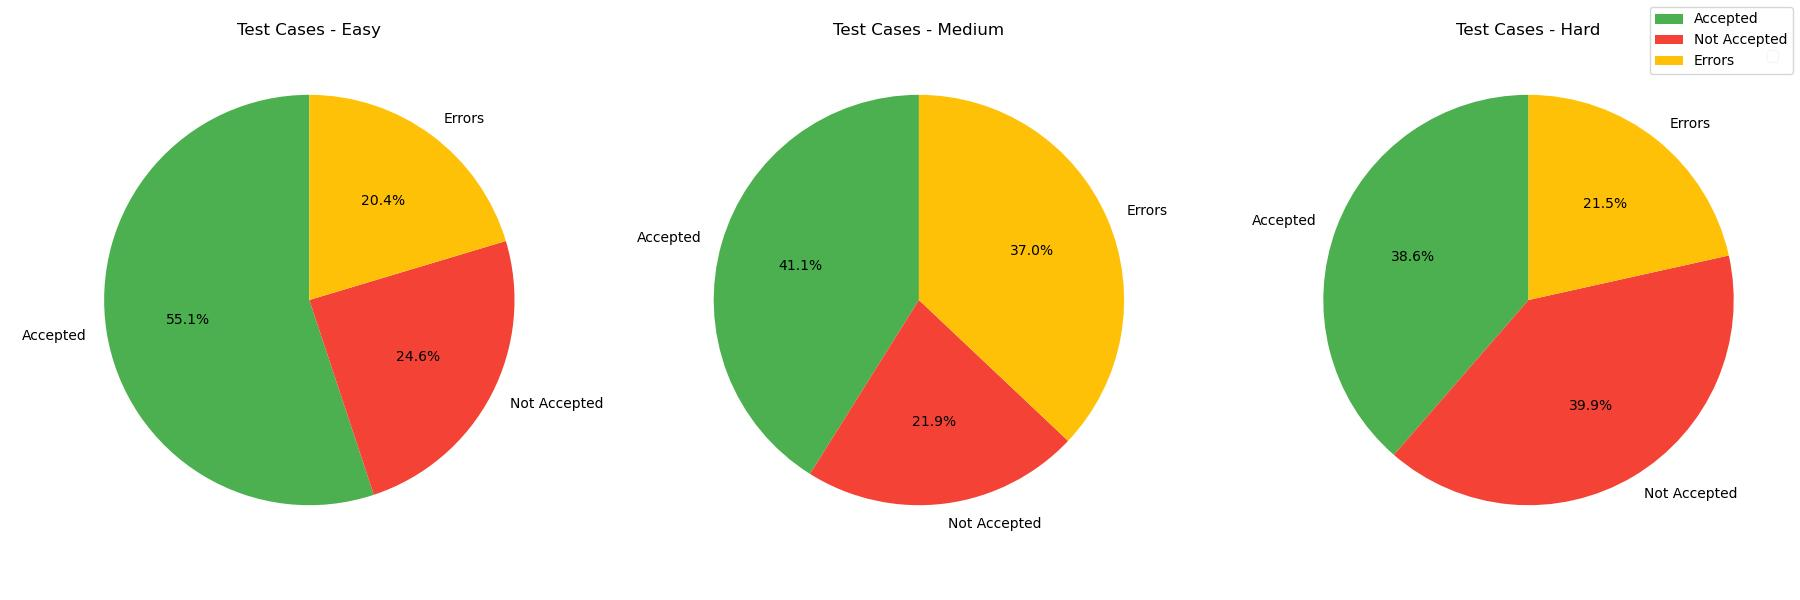
\includegraphics[width=1\textwidth]{figures/6/pie_difficulty.jpg}
    \caption{Distribution of test case results by difficulty level for Prompt 6}
    \label{fig:prompt6_difficulty}
\end{figure}

\begin{figure}[H]
    \centering
    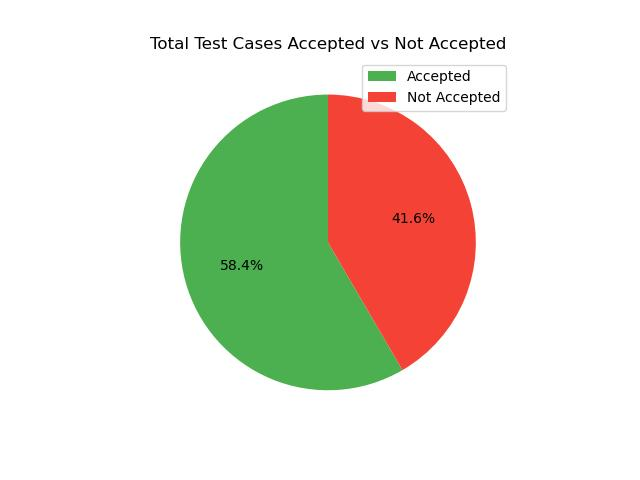
\includegraphics[width=0.8\textwidth]{figures/7/total_accepted_not.jpg}
    \caption{Performance breakdown for Prompt 7}
    \label{fig:prompt7_performance}
\end{figure}

\begin{figure}[H]
    \centering
    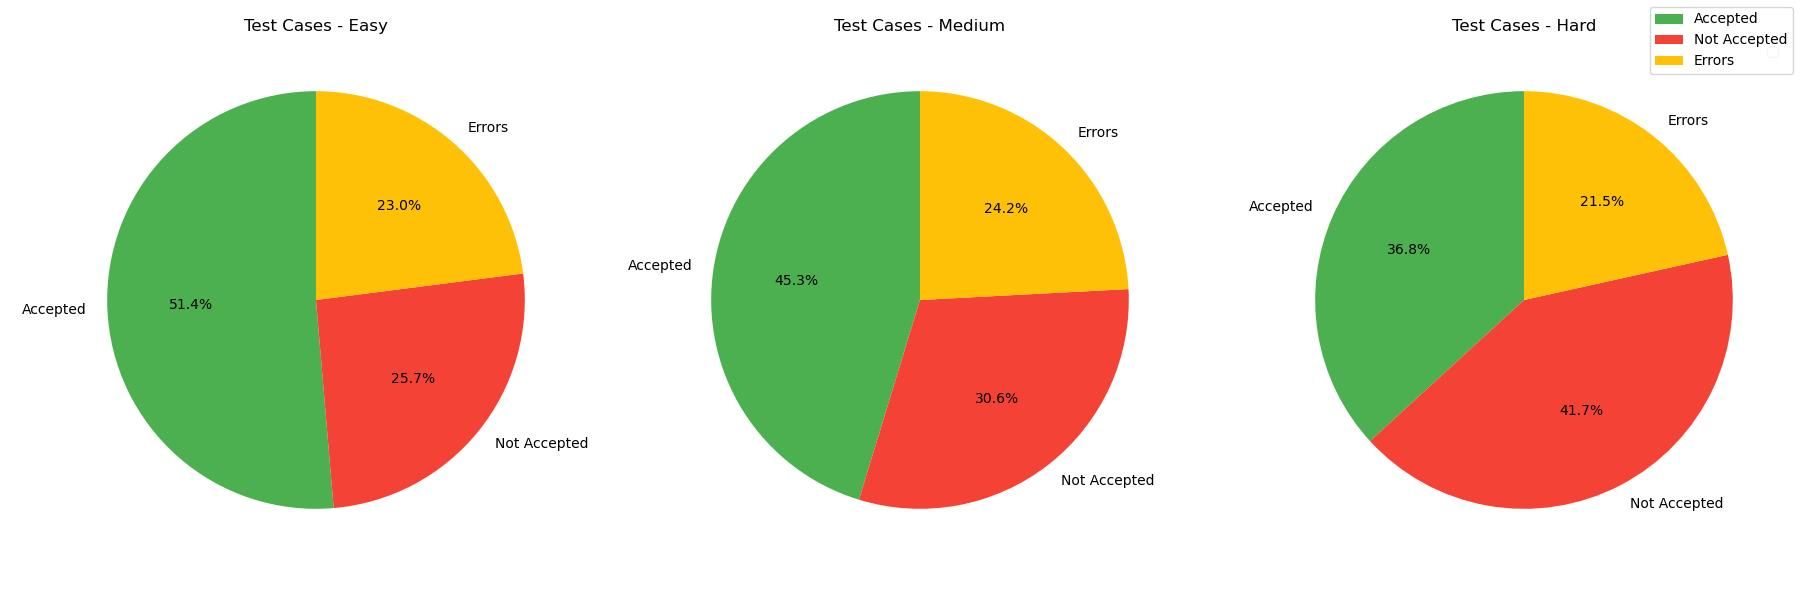
\includegraphics[width=1\textwidth]{figures/7/pie_difficulty.jpg}
    \caption{Distribution of test case results by difficulty level for Prompt 7}
    \label{fig:prompt7_difficulty}
\end{figure}

\begin{figure}[H]
    \centering
    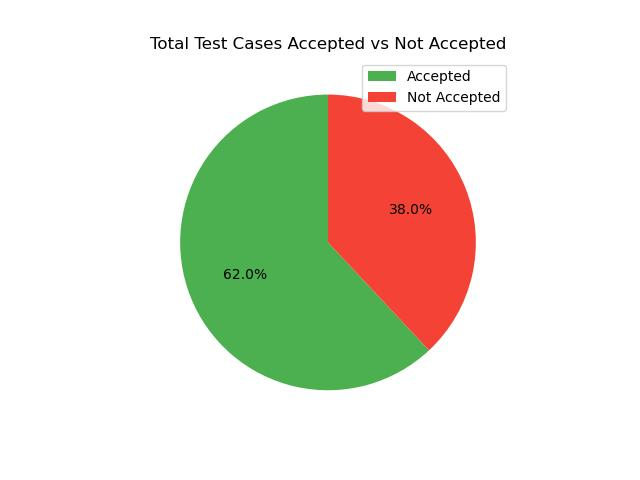
\includegraphics[width=0.8\textwidth]{figures/8/total_accepted_not.jpg}
    \caption{Performance breakdown for Prompt 8}
    \label{fig:prompt8_performance}
\end{figure}

\begin{figure}[H]
    \centering
    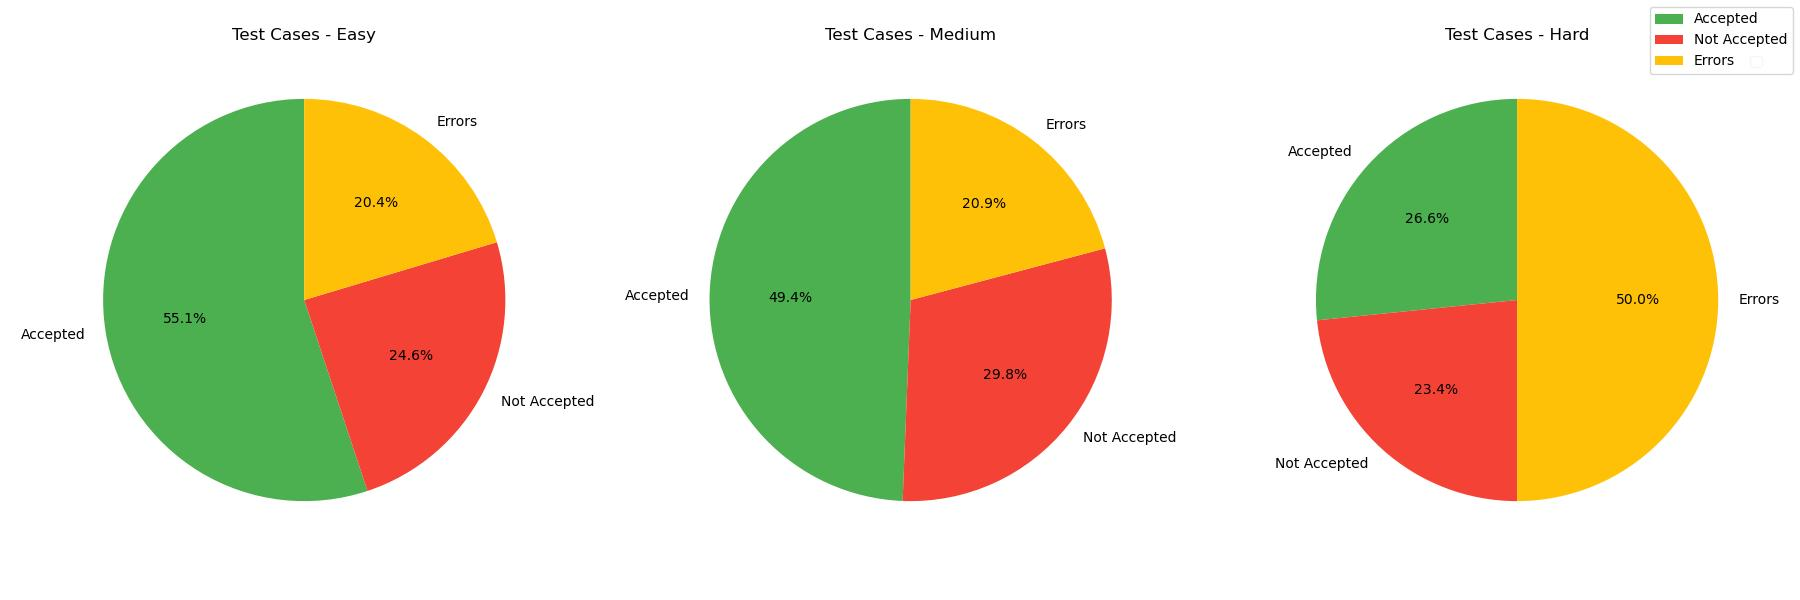
\includegraphics[width=1\textwidth]{figures/8/pie_difficulty.jpg}
    \caption{Distribution of test case results by difficulty level for Prompt 8}
    \label{fig:prompt8_difficulty}
\end{figure}

\begin{figure}[H]
    \centering
    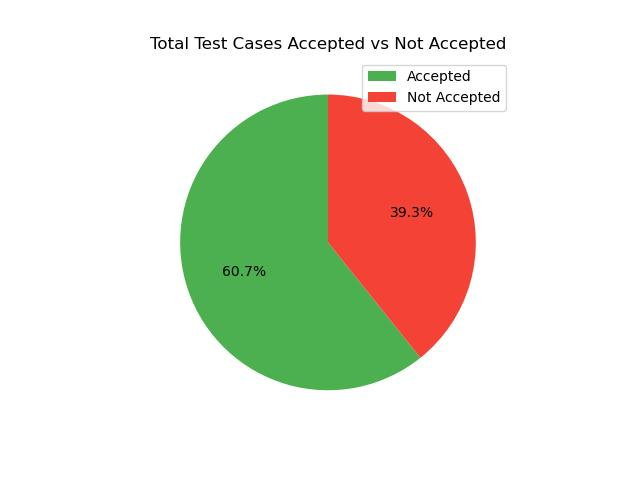
\includegraphics[width=0.8\textwidth]{figures/9/total_accepted_not.jpg}
    \caption{Performance breakdown for Prompt 9}
    \label{fig:prompt9_performance}
\end{figure}

\begin{figure}[H]
    \centering
    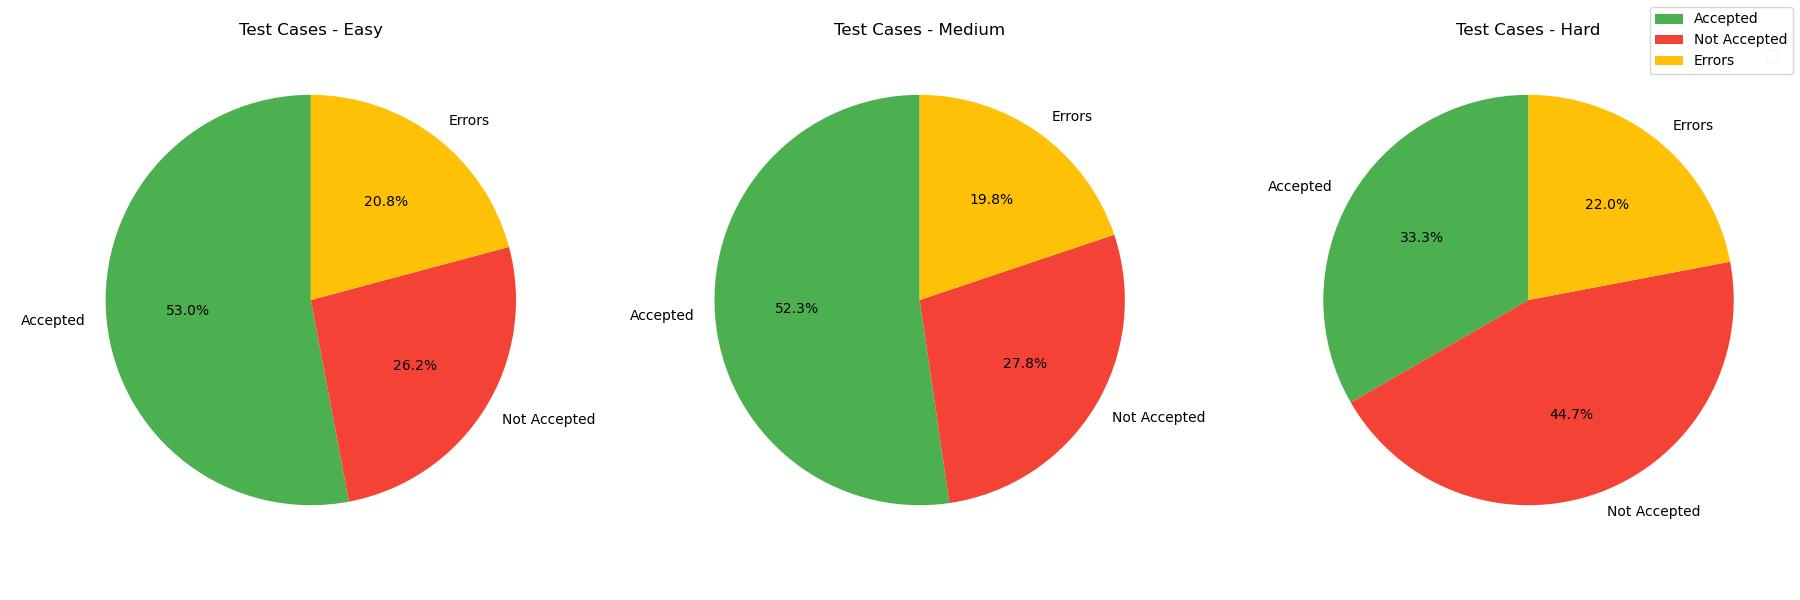
\includegraphics[width=1\textwidth]{figures/9/pie_difficulty.jpg}
    \caption{Distribution of test case results by difficulty level for Prompt 9}
    \label{fig:prompt9_difficulty}
\end{figure}

\subsection{Observing erroneous patterns}
The following figures ~\ref{fig:prompt1_difficulty}, ~\ref{fig:prompt2_difficulty}, ~\ref{fig:prompt3_difficulty}, ~\ref{fig:prompt4_difficulty}, ~\ref{fig:prompt5_difficulty}, ~\ref{fig:prompt6_difficulty}, ~\ref{fig:prompt7_difficulty}, ~\ref{fig:prompt8_difficulty}, ~\ref{fig:prompt9_difficulty} reveal the erroneous code generation which leads to failure. A simple correlation can be observed between the total number of errors to the overall acceptance rate. This suggests that guiding ChatGPT to produce less errors can be the key to unlocking higher orders of performance. Further study and analysis needs to be done to identify the causes for errors and the effect of prompting in guiding the model to produce error free code. 

\section{Summary}
The results presented in this chapter reveal significant insights into the effectiveness of different prompts in guiding ChatGPT to successfully solve DSA problems. The analysis indicates that specific prompts, especially those requiring concise and precise code solutions, tend to yield higher acceptance rates. This chapter sets the stage for a deeper discussion on the implications of these findings, which will be explored in the subsequent chapters of the thesis. For a detailed analysis of acceptance rates per topic for each prompt, refer to Appendix A.
